\documentclass[12pt]{article}
\usepackage[spanish,es-nodecimaldot]{babel}
\usepackage[utf8]{inputenc}
\usepackage[T1]{fontenc}
\usepackage[a4paper,margin=2.5cm]{geometry}
\usepackage{lmodern}
\usepackage{setspace}
\usepackage{parskip}
\usepackage{graphicx}
\usepackage{float}

\begin{document}
\thispagestyle{empty}

\begin{center}
    \textsc{Universidad Central de Venezuela}\\[0.35cm]
    \textsc{Facultad de Ingenier\'ia}\\[0.35cm]
    \textsc{Escuela de Ingenier\'ia El\'ectrica}\\[0.35cm]
    \textsc{Departamento de Potencia}\\[0.35cm]
    \textsc{Laboratorio de M\'aquinas El\'ectricas I}
\end{center}

\vspace{6.8cm}

\begin{center}
    \textbf{PRE-LABORATORIO N\textsuperscript{o}5}\\[0.35cm]
    \textbf{Transformador Monof\'asico. Comportamiento}
\end{center}

\vfill

\noindent
\begin{minipage}[t]{0.48\textwidth}
    Docente:\\[0.25cm]
    Blondell, Jes\'us
\end{minipage}%
\hfill
\begin{minipage}[t]{0.48\textwidth}
    \raggedleft
    Autor:\\[0.25cm]
    Br. Carla Fajardo\\[0.25cm]
    V-27.571.576
\end{minipage}

\vspace{1.1cm}

\begin{center}
    Caracas, 11 de septiembre de 2026
\end{center}

\newpage

\section{Introducci\'on}
El transformador monof\'asico es una m\'aquina el\'ectrica est\'atica utilizada para transferir energ\'ia entre dos circuitos mediante inducci\'on electromagn\'etica. Su funcionamiento permite modificar los niveles de tensi\'on y corriente de un sistema de corriente alterna, manteniendo la frecuencia de alimentaci\'on. 

En esta pr\'actica se estudiar\'a experimentalmente el comportamiento del transformador al alimentar diferentes tipos de carga. Inicialmente, se emplear\'a una carga resistiva o lineal, variando sus niveles para obtener mediciones de tensi\'on, corriente y potencia en los lados de baja y alta tensi\'on. Estos resultados permitir\'an observar la variaci\'on de la tensi\'on secundaria con la carga y evaluar la respuesta del transformador bajo condiciones aproximadamente lineales.

Posteriormente, se incorporar\'a un puente rectificador para alimentar una carga no lineal. En este caso, adem\'as de registrar los par\'ametros el\'ectricos, se observar\'an las formas de onda mediante el osciloscopio y se analizar\'an los efectos de la distorsi\'on y los arm\'onicos sobre la corriente, la tensi\'on y las p\'erdidas del transformador.

El an\'alisis de su comportamiento es fundamental para comprender la relaci\'on entre las variables el\'ectricas del primario y del secundario, as\'i como los efectos de las p\'erdidas, las impedancias internas y la regulaci\'on de tensi\'on.
\newpage

\section{Objetivos}
\subsection*{Objetivo General}
Estudiar el comportamiento de las variables e\'ectricas de un transformador monof\'asico cuando alimenta cargas lineales y no lineales.

\subsection*{Objetivos Espec\'ificos}
\begin{itemize}
    \item Obtener y evaluar experimentalmente la curva de carga $V_2 = f(I_2)$ operando el transformador con una carga lineal (resistencia variable).
    \item Medir las potencias activa y aparente y las formas de onda de tensión y corriente, tanto en la carga como en el lado primario del transformador para cargas no lineales.
    \item Comparar los resultados teóricos con las mediciones obtenidas en el laboratorio.
\end{itemize}

\newpage

\section{Marco te\'orico}
\subsection{Comportamiento del Transformador Monof\'asico}

\subsubsection*{Concepto y Principio de Funcionamiento}
\begin{itemize}
    \item El transformador monof\'asico es una m\'aquina el\'ectrica est\'atica alimentada con corriente alterna, compuesta por dos devanados (primario y secundario) arrollados sobre un n\'ucleo magn\'etico cerrado com\'un. Su funci\'on principal es transformar la energ\'ia el\'ectrica de c.a., modificando los valores de tensi\'on e intensidad de corriente de entrada a otros valores de salida.
\end{itemize}

\subsubsection*{Modelo ideal}
\begin{itemize}
    \item \textbf{Hip\'otesis del modelo:} Se asume que no existen p\'erdidas en el hierro ($P_{Fe}=0$), las resistencias de los devanados son nulas ($R_1=R_2=0$) y no hay flujos de dispersi\'on (todo el flujo magn\'etico permanece confinado dentro del n\'ucleo y enlaza a ambos devanados).

    \item \textbf{Relaci\'on de transformaci\'on ($m$ o $a$):} La relaci\'on entre las tensiones en bornes, las fuerzas electromotrices (f.e.m.) e idealmente el n\'umero de espiras viene dada por:
    \[
        \frac{V_1}{V_2}=\frac{E_1}{E_2}=\frac{N_1}{N_2}=m \quad (o\ a)
    \]

    \item \textbf{Relaci\'on de corrientes:} Las corrientes se transforman en proporci\'on inversa al n\'umero de espiras:
    \[
        \frac{I_1}{I_2}=\frac{N_2}{N_1}=\frac{1}{m}
    \]

    \item \textbf{Transformaci\'on de impedancias:} Cualquier impedancia $Z_2$ conectada al secundario se refleja o refiere al primario multiplicada por el cuadrado de la relaci\'on de transformaci\'on:
    \[
        Z_1=m^2Z_2
    \]
\end{itemize}

\subsubsection*{Funcionamiento en Vac\'io (Sin Carga, $I_2=0$)}
\begin{itemize}
    \item Al aplicar tensi\'on en el primario manteniendo el secundario abierto, el transformador se comporta como una bobina con n\'ucleo de hierro y absorbe una peque\~na \textbf{corriente de vac\'io o excitaci\'on} ($I_0$ o $I_{0ex}$).

    \item Esta corriente consta de dos componentes fasoriales:
    \begin{enumerate}
        \item \textbf{Componente magnetizante ($I_{m}$ o $I_{\mu}$):} Encargada de crear el flujo magn\'etico en el n\'ucleo, desfasada 90 grados en retraso respecto a la f.e.m. inducida.
        \item \textbf{Componente de p\'erdidas en el hierro ($I_{Fe}$ o $I_c$):} En fase con la f.e.m. inducida, orientada a suministrar la potencia activa absorbida por el n\'ucleo (hist\'eresis y corrientes par\'asitas o de Foucault).
    \end{enumerate}
\end{itemize}

\subsubsection*{Funcionamiento en Carga ($I_2>0$)}
\begin{itemize}
    \item Al conectar una carga al secundario, circula una corriente $I_2$ que genera una fuerza magnetomotriz (f.m.m.) $N_2I_2$ desmagnetizante.

    \item Para mantener el flujo en el n\'ucleo pr\'acticamente constante, el primario absorbe autom\'aticamente de la red una componente de corriente de carga $I'_1$ tal que se equilibren las f.m.m. ($N_1I'_1=N_2I_2$).

    \item La corriente primaria total es la suma fasorial de la corriente de vac\'io y la de carga:
    \[
        I_1=I_0+I'_1
    \]
\end{itemize}

\subsubsection*{Transformador Real}
\begin{itemize}
    \item En la pr\'actica, intervienen las resistencias el\'ectricas de los conductores ($R_1$, $R_2$) y los flujos de dispersi\'on (que completan su circuito por el aire) representados por las reactancias de dispersi\'on ($X_1$, $X_2$).

    \item Estas impedancias internas provocan ca\'idas de tensi\'on que hacen que la tensi\'on secundaria var\'ie con la magnitud de la carga y su factor de potencia (\textbf{regulaci\'on de tensi\'on}).
\end{itemize}

\subsection{Comportamiento del Transformador con Cargas Lineales y No Lineales}

\subsubsection*{Cargas Lineales y Comportamiento Ideal/Lineal}
\begin{itemize}
    \item \textbf{Linealidad ideal:} Si el circuito magn\'etico tuviera una permeabilidad constante y la carga conectada fuera lineal (resistencias, inductancias o capacitancias puras con impedancia constante), al aplicar una tensi\'on sinusoidal las corrientes y tensiones secundarias responder\'ian con ondas sinusoidales proporcionales.

    \item \textbf{Respuesta en el tiempo:} Las magnitudes se mantienen puramente sinusoidales a la frecuencia de la red, variando \'unicamente el desfase fasorial de la corriente seg\'un el factor de potencia de la carga (inductivo, capacitivo o unitario).
\end{itemize}

\subsubsection*{Cargas No Lineales y Saturaci\'on del N\'ucleo}
\begin{itemize}
    \item \textbf{No linealidad inherente del n\'ucleo ferromagn\'etico:} A causa de la hist\'eresis y la saturaci\'on de la curva de magnetizaci\'on del hierro, el transformador es en s\'i un dispositivo no lineal. Incluso alimentando cargas lineales o en condici\'on de vac\'io, la corriente de excitaci\'on se deforma adoptando una forma no sinusoidal con presencia de arm\'onicos impares (con una presencia predominante del 3.er arm\'onico).

    \item \textbf{Efectos de las Cargas No Lineales (electr\'onica de potencia, rectificadores, etc.):}
    \begin{enumerate}
        \item \textbf{Generaci\'on e inyecci\'on de arm\'onicos de corriente:} Dispositivos no lineales (como rectificadores o convertidores controlados) absorben corrientes pulsantes y no sinusoidales compuestas por una onda fundamental y m\'ultiples arm\'onicos.

        \item \textbf{Deformaci\'on de la tensi\'on de la red:} La circulaci\'on de los arm\'onicos de corriente a trav\'es de las reactancias e impedancias de dispersi\'on del transformador genera ca\'idas de tensi\'on arm\'onicas que deforman la onda de tensi\'on terminal.

        \item \textbf{Aumento de p\'erdidas y calentamiento:} Los arm\'onicos de corriente de alta frecuencia causan un incremento de las p\'erdidas por efecto Joule ($I^2R$) en las bobinas y aumentan dr\'asticamente las p\'erdidas en el n\'ucleo por corrientes par\'asitas y saturaci\'on.

        \item \textbf{Saturaci\'on por componente continua (c.c.):} Algunos circuitos rectificadores no sim\'etricos (como los de media onda) introducen una componente continua de corriente en el secundario, lo que induce saturaci\'on continua en el n\'ucleo magn\'etico. Para prevenirlo, los transformadores para cargas no lineales requieren ser dise\~nados con inducciones m\'as bajas y factores de utilizaci\'on calculados espec\'ificamente para estas condiciones.

        \item \textbf{Deformaci\'on del flujo y neutro flotante:} Si el sistema o la conexi\'on del transformador restringe la libre circulaci\'on de los arm\'onicos de corriente necesarios (por ejemplo, en bancos estrella-estrella de tres hilos sin neutro), la corriente se fuerza a ser sinusoidal y se deforma el flujo magn\'etico, originando arm\'onicos en las tensiones de fase, sobretensiones y la oscilaci\'on del neutro (``neutro inquieto'').
    \end{enumerate}
\end{itemize}

\newpage

\section{Equipos e instrumentos}
\begin{itemize}
    \item Transformador monof\'asico.
    \item Variac.
    \item Vat\'imetro.
    \item Volt\'imetro de hierro m\'ovil.
    \item Amper\'imetro de hierro m\'ovil.
    \item Osciloscopio digital.
    \item Puente rectificador.
    \item Fuente de alimentaci\'on AC.
    \item Resistencia shunt.
    \item Carga lineal.
    \item Carga no lineal.
    \item Cables de conexi\'on.
    \item Interruptor de prueba.
\end{itemize}

\section{Diagrama de un transformador monof\'asico\\con carga resistiva}
\begin{figure}[H]
    \centering
    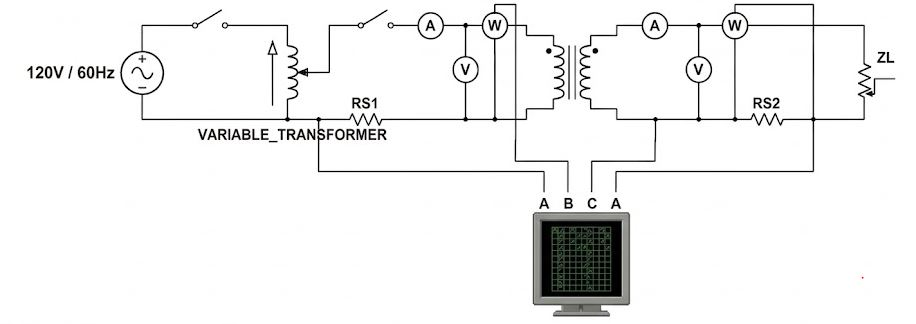
\includegraphics[width=\textwidth]{pre5_1.JPG}
    \caption{Diagrama de un transformador monof\'asico con carga resistiva.}
\end{figure}

\begin{figure}[H]
    \centering
    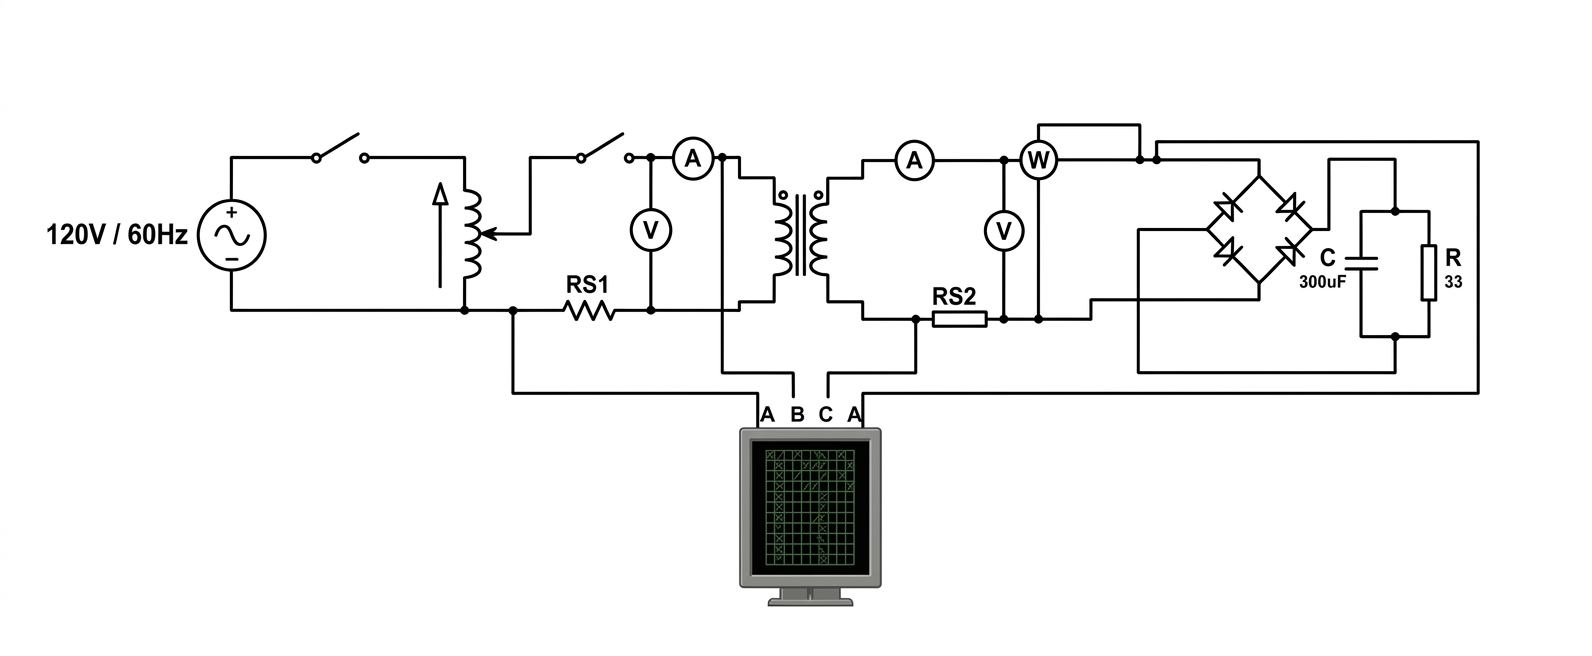
\includegraphics[width=\textwidth]{gemini_generator.jpg}
    \caption{Diagrama de un transformador con rectificador y carga no lineal.}
\end{figure}

\section{Metodolog\'ia}
Para el desarrollo de la pr\'actica, se llevar\'a a cabo el siguiente procedimiento:

\begin{enumerate}
    \item \textbf{Montaje del Circuito:}
    \begin{itemize}
        \item Se realizar\'a el montaje siguiendo el esquema de conexi\'on de la Figura 1. 
        \item Luego se conectar\'a el osciloscopio empleando resistencias shunt ($R_s$) para la visualizaci\'on de las formas de onda del voltaje y la corriente.
    \end{itemize}

    \item \textbf{Ensayo con Carga Lineal:}
    \begin{itemize}
        \item Se energizar\'a el circuito ajustando el VARIAC hasta obtener la tensi\'on nominal.
        \item Luego se proceder\'a a variar la carga resistiva en distintos niveles, registrando los valores de tensi\'on ($V_2$), corriente ($A_2$) y potencia activa ($W_2$).
        \item Adem\'as de tomar'an fotos de las formas de onda de tensi\'on y corriente observadas en el osciloscopio.
    \end{itemize}

    \item \textbf{Ensayo con Carga No Lineal:}
    \begin{itemize}
        \item Se intercalar\'a el puente rectificador en el lado secundario del transformador para alimentar la carga no lineal.
        \item Luego se toma\'an las mediciones de los par\'ametros observando la distorsi\'on inducida en la se\~nal.
        \item Por \'utimo se ajustar\'an los elementos de la carga y se documentar\'an las variaciones en el factor de potencia y los arm\'onicos.
    \end{itemize}
\end{enumerate}

\section{Resultados}
\begin{center}
    \textbf{Mediciones bajo carga resistiva (lineal) en el transformador}

    \vspace{0.25cm}
    \small
    \renewcommand{\arraystretch}{1.25}
    \begin{tabular}{|c|ccc|ccc|}
        \hline
        \multicolumn{1}{|c|}{\textbf{Carga [W]}} & \multicolumn{3}{c|}{\textbf{Baja Tensi\'on}} & \multicolumn{3}{c|}{\textbf{Alta Tensi\'on}} \\
        \hline
        & $V_1$ [V] & $I_1$ [A] & $P_1$ [W] & $V_2$ [V] & $I_2$ [A] & $P_2$ [W] \\
        \hline
         & & & & & & \\
         & & & & & & \\
         & & & & & & \\
         & & & & & & \\
         & & & & & & \\
         & & & & & & \\
         & & & & & & \\
         & & & & & & \\
         & & & & & & \\
         & & & & & & \\
        \hline
    \end{tabular}
\end{center}

\vspace{0.5cm}

\begin{center}
    \small
    \renewcommand{\arraystretch}{1.25}
    \begin{tabular}{|cc|ccc|}
        \hline
        \multicolumn{2}{|c|}{\textbf{Baja Tensi\'on}} & \multicolumn{3}{c|}{\textbf{Alta Tensi\'on}} \\
        \hline
        $V_1$ [V] & $I_1$ [A] & $V_2$ [V] & $I_2$ [A] & $P_2$ [W] \\
        \hline
        \hline
    \end{tabular}
\end{center}

\vspace{0.5cm}

\begin{center}
    \small
    \renewcommand{\arraystretch}{1.25}
    \begin{tabular}{|c|cc|ccc|}
        \hline
        \textbf{Carga [W]} & \multicolumn{2}{c|}{\textbf{Baja Tensi\'on}} & \multicolumn{3}{c|}{\textbf{Alta Tensi\'on}} \\
        \hline
        & $V_1$ [V] & $I_1$ [A] & $V_2$ [V] & $I_2$ [A] & $P_2$ [W] \\
        \hline
        \hline
    \end{tabular}
\end{center}

\newpage

\section{Referencias}
\begin{enumerate}
    \item Nerio Ojeda, Juli\'an P\'erez. \textit{Pr\'actica 4. Transformador Monof\'asico. Modelo}. Universidad Central de Venezuela, Facultad de Ingenier\'ia, Escuela de Ingenier\'ia El\'ectrica, Departamento de Potencia, Laboratorio de M\'aquinas I, Revisi\'on 2012.
    \item Fraile Mora, Jes\'us. \textit{M\'aquinas El\'ectricas} (6\textsuperscript{a} Ed.). McGraw-Hill, 2008.
    \item S. J. Chapman, \textit{M\'aquinas el\'ectricas}, 5ta ed. M\'exico D.F.: McGraw-Hill, 2012. (Referencia est\'andar para el funcionamiento, circuito equivalente y regulaci\'on de tensi\'on).
\end{enumerate}

\end{document}
